\chapter{Arkitektur}
 Projektet er forsøgt at blive designet på en måde hvor så mange dele af projektet er udskiftelige så muligt.

\section{Lagmodel}
I Projektet er der anvendt en lagdelt arkitektur, som er opdelt i tre lag. De tre lag er Presentations, Buisness logik  og Data access.  

\subsection{Presentationlag}
\subsection{Buisness logik lag}
\subsection{Data Acces lag}





\section{Teknologivalg}

Til Bargainbarter er der valgt en række teknologier, hvor enkelte har større indflydelse end andre på det samlede project. Nedenfor beskrives de enkelte teknologivalg, og begrundelsen for valget.

\subsection{ASP.Net MVC}
Da projektet der udvikles er en webapplication og undervisningen til individerne i gruppen, foregår i C\# var ASP.Net MVC det oplagte valg, som mødte gruppens krav om at tilbyde webudvikling. Microsoft web frameworket er opbygget udfra et MVC pattern, som er eksemplificeret på fig. \ref{fig:MVC}.

\begin{figure}[H]
	\centering
	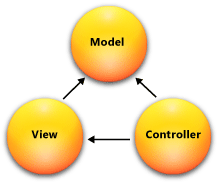
\includegraphics
	[width=165mm]{figures/MVC.png}
	\caption{BILLEDET ER FORKERT}
	\label{fig:MVC}
\end{figure}     

På fig. \ref{fig:MVC} ses at projektets views skal opdateres og gives til brugeren gennem controllerne. Disse kontrollere kaldes igennem url'en som en http protocol, og returnere web sider til clienten, mens modellen reprensentere de data der er i projektet. Denne model opdateres ligeledes igennem controllerne.   

\subsection{Entityframwork}
Entity frameworked var det oplagte valg når først ASP.Net MVC var valgt. EF kommer som standard når der oprettes et ASP.net mvc projekt, og opretter selv en skabelon at bruge det ud fra. Desuden for gruppen sidst på semesteret undervisning i EF og der var derfor ingen tvivl. EF er en ORM der giver mulighed for at lave og vedligeholde en database, men på objektorienteret vis. For fuld beskrivelse af EF og brugen af det i projektet, se Dokumenationen.

\subsection{webteknology}
Igennem selve viewet der sendes til clienterne af BargainBarter, er der brugt HTML, CSS , javascript inkl. JQuery, signalR, bootstrap. Der gives ingen videre forklaring på valget af disse, da de er rimeligt nødvendige i webudvikling
 